\section{Preliminaries}
Let $\vecs\xi \in \mathbb{R}^N$ describe the system's state in an $N \geq 2$ dimensional space, e.g., the robot's joint or Cartesian space positions.
The function $\vecs f(\vecs \xi): \mathbb{R}^N \rightarrow \mathbb{R}^N$ represents a smoothly defined dynamical system (DS) describing the desired velocity at a given state $\vecs \xi$.  
The first and second-order time derivatives are denoted by one and two dots over the symbol respectively, i.e., $\dot{\vecs \xi} =\frac{d}{dt} \vecs \xi$ is the systems velocity, and $\ddot{\vecs \xi} = \frac{d^2}{dt^2} \vecs \xi$ is the acceleration.
In general, superscripts are used for variable names, whereas subscripts are used for enumerations.
%Furthermore, all trajectories converge to the unique attractor state $\vecs \xi ^a \in \mathbb{R}^N$. 

\subsection{Obstacle Avoidance}
Let us assume the base velocity $\vect f^b(\vecs \xi): \mathbb{R}^N \rightarrow \mathbb{R}^N$, which describes the desired, state-dependent motion of the robot. 
As proposed by \cite{huber2019avoidance, huber2022avoiding}, an obstacle avoiding velocity $\vect f(\vecs \xi): \mathbb{R}^N \rightarrow \mathbb{R}^N$ can be achieved by a simple matrix multiplication (or modulation) as follows:
\begin{equation}
\begin{split}
  & \vecs f(\vecs \xi) = \textbf{E}(\vecs \xi) \text{diag} \left(\lambda^r, \lambda^e, ..., \lambda^e \right) \textbf{E}(\vecs{\xi})^{-1} \vect f^b(\vecs \xi) \\
  % \label{eq:modulated_ds}
% \end{equation}
%
%The orthonormal basis matrix $\textbf{E} \in \mathbb{R}^{N \times N}$, defined as:
%\begin{equation}
& \text{with} \quad
\textbf{E}(\vecs \xi) = \left[ \textbf{r}(\vecs \xi) \ \textbf{e}_1(\vecs \xi) \ ... \ \textbf{e}_{d-1}(\vecs \xi) \right]
%\label{eq:matrix_E}
\end{split}
  \label{eq:modulated_ds}
\end{equation}
where the tangent directions $\textbf{e}_{(\cdot)} \in \mathbb{R}^N$ are perpendicular to the surface normal $\vect n(\vecs \xi) \in \mathbb{R}^N$, see Fig.~\ref{fig:resultant_normal}. The reference vector $\textbf{r}(\vect{\xi}) =  \left( \vecs{\xi}-\vecs{\xi}^r \right) / \| \vecs \xi-\vecs \xi ^r \|$ is pointing towards the the reference point $\vecs \xi^r \in \mathbb{R}^N$. 
This construction of the basis matrix is valid for starshaped obstacles, i.e., shapes for which a reference point exists, from which a line in any direction only crosses the surface once \cite{huber2023avoidance}.

The diagonal values $\lambda_{(\cdot)}$ in \eqref{eq:modulated_ds} are often referred to as eigenvalues since they modify the length of the input velocity in specific directions. 
The eigenvalue in reference direction $\lambda^r(\vecs \xi) \leq 1$, is designed to reduce the velocity towards the obstacle.  
Conversely, the velocity increases along the tangent direction using $\lambda^e(\vecs \xi) \geq 1$. The eigenvalues in reference direction $\lambda^r$ and tangent direction $\lambda^e$ are defined as:
\begin{equation}
\begin{split}
    \lambda^r(\vecs \xi) = 1 - 1 /\Gamma(\vecs \xi) , \quad \lambda^e(\vecs \xi) = 1 + 1 / \Gamma(\vecs \xi)
    \label{eq:eigenvalues}
    \end{split}
\end{equation}
with the continuous distance function $\Gamma(\vecs \xi) \in \mathbb{R}_{\geq 0}$, which has a value of $\Gamma(\vecs \xi) = 1$ on the boundary of an obstacle, and monotonically increases along the normal to the surface of the obstacle (Fig.~\ref{fig:resultant_normal}). In this work, we use:
\begin{equation}
  \Gamma(\vecs \xi) = 1 + \| \vecs \xi - \vecs \xi^b \|  / R^0
  \quad \text{with} \quad
  \vecs \xi^b = b (\vecs \xi - \vecs \xi^r) + \vecs \xi^r
  \label{eq:distance_function}
\end{equation}
with $b \in \mathbb{R}_{>0}$, such that $\vect \xi^b \in \mathbb{R}^N$ lies on the surface of the obstacle, and $R^0 \in \mathbb{R})_{>0}$ is the distance scaling, we use $R^0 = 1$.

\begin{figure}
\iflong
\centerline{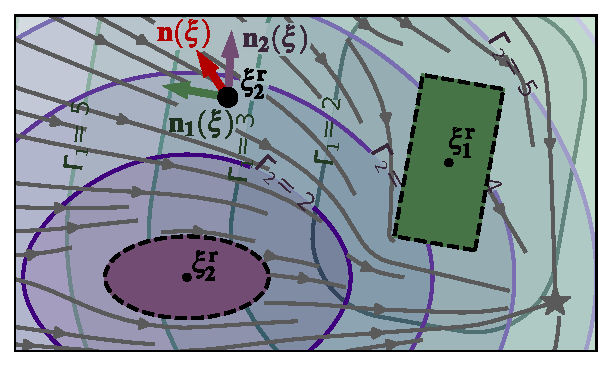
\includegraphics[width=0.8\columnwidth]{figures/normal_and_gamma_field_visualization_annotated.pdf}}
\else
\centerline{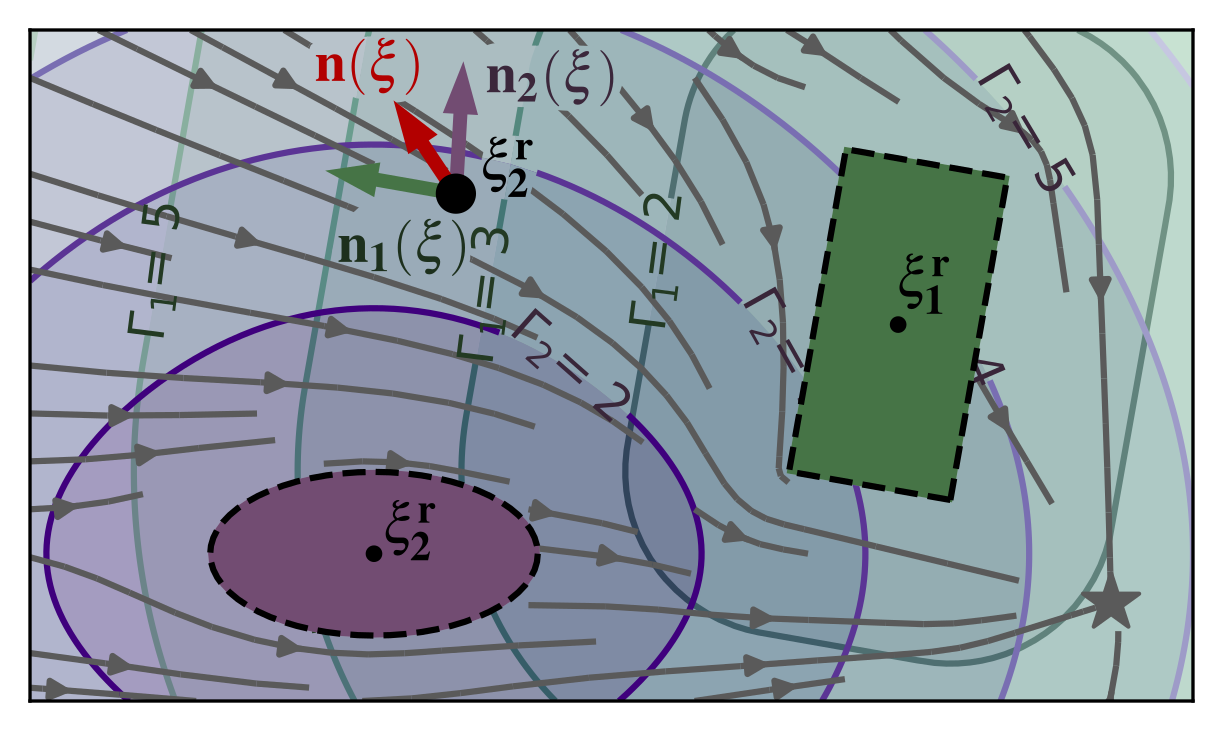
\includegraphics[width=0.8\columnwidth]{figures/normal_and_gamma_field_visualization_annotated.png}}
\fi
\caption{
The $\Gamma$-field is defined individually for each of the obstacles. At each position $\vecs \xi$, we can evaluate the surface normal $\vect n(\vecs \xi)$. 
The velocity $\vect f(\vecs \xi)$ (gray) avoids collision with the obstacles and converges towards the attractor (star).}
\label{fig:resultant_normal}
\end{figure}

\iflong
Modifying the base velocity $\vect f^b(\vecs \xi)$ with these eigenvalues values and \eqref{eq:modulated_ds} leads to obstacle-avoiding dynamics $\vect f(\vecs \xi)$ which generate converging motion around starshaped obstacles.
\fi

\subsection{Force Control}

\subsubsection{Rigid Body Dynamics}
A force-controlled system is subject to acceleration, inertia, and external disturbances. Its general rigid-body dynamics based on the state $\vecs \xi$ are given as
\begin{equation}
\matd{M}(\vecs\xi)\vecs{\ddot\xi} + \matd{C}(\vecs\xi, \vecs{\dot\xi})\vecs{\dot\xi} + \vect g(\vecs\xi) = \vecs{\tau_c} + \vecs{\tau_e}
 \label{eq:robot_dynamics}
\end{equation}
where we have the mass matrix of the robot $\matd M(\vecs\xi) \in \mathbb{R}^{N \times N}$, the Coriolis matrix $\matd C(\vecs\xi,\vecs{\dot\xi}) \in \mathbb{R}^N$, the gravity vector $\vect g(\vecs\xi) \in \mathbb{R}^N)$, the control torque $\vecs{\tau_c} \in \mathbb{R}^N$, and the external torque, also referred as disturbance, $\vecs{\tau_e} \in \mathbb{R}^N$.

\subsubsection{Damping Controller}
Damping control \cite{kronander2015passive} offers a powerful method for computing control forces from a velocity field. This controller provides selective disturbance rejection based on the direction of the desired motion. Typically, the controller is configured with high damping along the direction of motion, ensuring rapid convergence of the robot's velocity to the desired value and achieving excellent tracking performance. In contrast, the controller exhibits high compliance in the direction perpendicular to the motion, enabling flexible behavior and greater resistance to external forces. The passive control force is evaluated as follows:
\begin{equation}
	\vecs{\tau_c} = \vect g (\vecs\xi) 
	% + \matd{D}(\vect \xi, \dot{\vect \xi}) \dot{\vect \xi}  
	+ \matd{D}(\vecs\xi) \left(\vecs f(\vecs\xi) - \vecs{\dot\xi} \right) 
\label{eq:control_command}
\end{equation}
This control law embeds a gravity compensation term $\vect g (\vecs\xi) \in \mathbb{R}^N$ and a positive-definite damping term, which dampens the difference between the desired velocity $\vecs f(\vecs\xi)$ and the actual velocity $\vecs{\dot\xi}$.
The positive definite damping matrix $\matd D(\vecs\xi) \in \mathbb{R}^{N \times N}$ is given as:
\begin{equation}
   \matd {D}(\vecs \xi) = \matd{Q}(\vecs\xi)\matd{S}(\vecs\xi) \matd{Q} (\vecs \xi)^{-1}
\label{eq:damping_matrix}
\end{equation}
where $\matd Q(\vecs \xi) = \left[ \vecs{q}_1 \, , \; \vecs q_2\ , \; ... \, , \; \vecs q_N \right] $ is an orthonormal basis matrix, of which the first vector is pointing in the desired direction of motion
\begin{equation}
    \vecs q_1(\vecs \xi) = \vecs q_1^f(\vecs \xi) = \vect f({\vecs \xi}) / \lVert \vect f({\vecs \xi}) \rVert \label{eq:velocity_unit_vector}
\end{equation}

The diagonal matrix $\matd{S}(\vecs\xi) \in \mathbb{R}^{N \times N}$ consists of damping factors $s_i \in \mathbb{R}_{>0}$ in the corresponding direction $i = 1 .. N$.
This design allows the separate design of the damping in the direction of motion and perpendicular to the motion.
Increased consistency with the desired velocity is achieved by using a high value for the first damping factor. Conversely, the damping in the remaining directions is set lower to allow compliance perpendicular to the motion, i.e., $s_i / s_1 \ll 1, \; i = 2 .. N$.

\iflong
\subsection{Stability Analysis} \label{sec:trad_passive}
Considering varying control parameters carefully is crucial, as such a design can inject energy into a system, potentially leading to unstable behavior and damaging the system \cite{ferraguti2013tank}.
In human-robot interaction, the robot faces external disturbances of unknown nature. To achieve stable and bounded behavior in the face of such disturbances, \textit{passivity} analysis is a valuable tool. By employing passivity analysis, the control system can be designed to maintain stable responses (bounded system) in the presence of any external force (bounded input). 

\begin{definition}[Passivity \cite{willems1972dissipative, sepulchre2012constructive}] \label{def:passivity}
	A dynamical system with input $ u \in \mathcal{U}$ and output $y \in \mathcal{Y}$ is passive with respect to the supply rate $s : \mathcal{U} \times \mathcal{Y} \rightarrow{R}$ if, for any $u: \mathbb{R}_{>0} \rightarrow \mathcal{U}$ and any time $t^* \geq 0$ the following is satisfied
  \begin{equation}
	  \int_0^{t^*} s \left( u(t),  y (t) \right) d \tau \geq S(t^*) - S(0) 
  \end{equation}
  where $S(t) \in \mathbb{R}_{\geq 0}$ is the storage function.
\end{definition}

The feedback loop combining two passive systems results in a passive system \cite{sepulchre2012constructive}. Hence, if the controller is passive, its application to a (passive) environment-hardware system results in a passive system.
\fi
